\chapter{Návrh}
% TODO: dopsat úvodní text této kapitoly

\section{Návrh způsobu specifikace pravidel}

Abychom mohli specifikovat pravidla, musíme nejprve definovat strukturu, nad kterou budou tato pravidla platit. V~tomto textu formalizujeme model programu pomocí teorie grafů. Nad grafem je potom možné specifikovat pravidla, která musí vstupní projekt splňovat.

\subsection{Formalizace modelu programu pomocí grafu}
\label{design-graph_formalization}

Analyzovaný softwarový projekt abstrahujeme jako orientovaný multigraf rozšířený o~zobrazení množiny uzlů do množiny typů a zobrazení hran do množiny jejich klasifikátorů (označení typu vztahu mezi uzly). Dále přidáme ke každému vrcholu zobrazení, které mu přiřadí jméno (řetězec). Získáme tak následující strukturu:

\begin{displaymath}
  G = \langle V, E, \rho, K, C, N, \mathit{Kind}, \mathit{Classifier}, \mathit{Name}\rangle
  \label{extended_multigraph}
\end{displaymath}
v~níž platí:
\begin{itemize}
\item $V$ je množina elementů (v~našem případě části kódu)
\item $E$ je množina hran (v~našem případě vztahy mezi částmi kódu - např. volání funkce, dědičnost)
\item $V \cap E = \emptyset$
\item $\rho: E \mapsto V \times V$ je zobrazení množiny hran do množiny uspořádaných dvojic vrcholů (incidence)
\item $K$ je libovolná množina označení typů vrcholů\footnote{Pod pojmem typ zde rozumíme jakékoliv označení, které specifikuje o~jaký objekt se jedná -- může to být třída, metoda, příkaz, \ldots},
\item $\mathit{Kind}: V \mapsto K$ je zobrazení, které přiřadí každému vrcholu jeho typ,
\item $C$ je množina klasifikátorů hran,
\item $N$ je množina jmen (řetězců)
\item $\mathit{Classifier}: E \mapsto C$ je zobrazení, které přiřadí každé hraně její klasifikátor (zda se jedná o~\emph{method call}, \emph{dědičnost}, atd.)
\item $\mathit{Name}: V \mapsto N$ je zobrazení, které přiřadí vrcholu jeho jméno (např. jméno třídy, jméno metody, \ldots)
\end{itemize}

Ukázka formalizace zdrojového kódu pomocí grafu je na obrázku \ref{design-graph_example}. V~uvedeném příkladě můžeme strukturu $G$ namapovat následujícím způsobem:
\begin{figure}[h!]
  \centering
  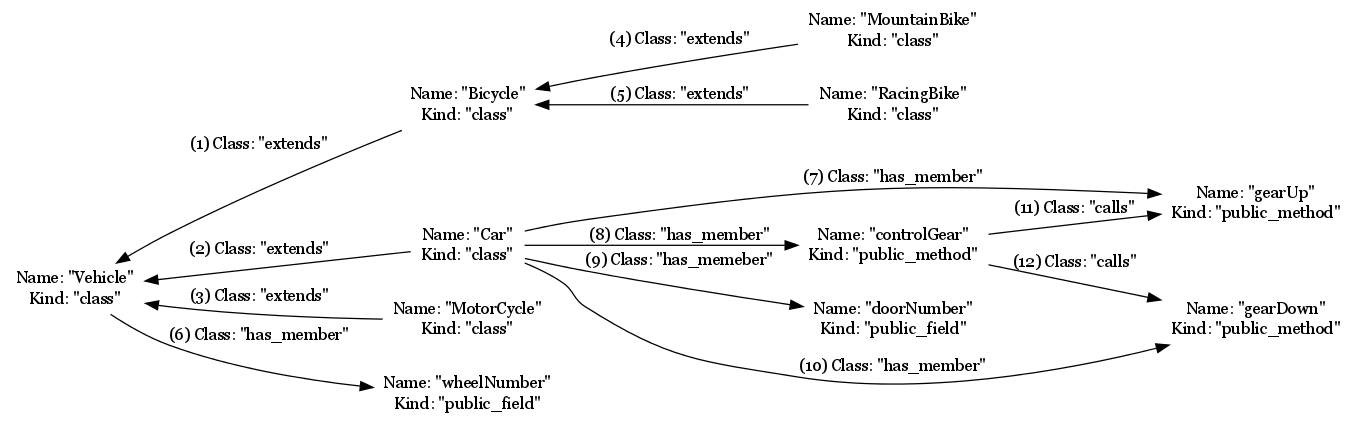
\includegraphics[width=1.0\textwidth]{./graphs/graph_example.png}
  \caption{Příklad formalizace hierarchie tříd jako grafu.\label{design-graph_example}}
\end{figure}
Množinu vrcholů můžeme ztotožnit s~množinou názvů elementů (v~našem případě třídy, pole, metody)\footnote{V konečném důsledku bude tato množina představována konkrétními elementy tak, jak se nalézají ve zdrojovém kódu.}.
\begin{align*}
  V~= &\{ \\
  &``Vehicle", ``Car", ``MotorCycle", ``Bicycle", ``MountainBike", ``RacingBike", \\
  &``wheelNumber", ``doorNumber", \\
  &``controlGear", ``gearUp", ``gearDown" \\
  &\}
\end{align*}
Abychom mohli demonstrovat množinu hran, bylo provedeno očíslování. Hranu zde identifikujeme číslem. V~počítačové reprezentaci se může jednat o~konkrétní objekt uložený v~poli. Zvolený identifikátor hrany nemá vliv na prováděnou analýzu, musí pouze zajistit jednoznačnou identifikaci hrany. Množinu hran zde v~textu reprezentujeme prostým výčtem čísel\footnote{V programu bude potom hrana reprezentována konkrétním objektem případně rozšířeným o~vhodný jedinečný identifikátor.}:

\begin{displaymath}
  E = \{1, 2, 3, 4, 5, 6, 7, 8, 9, 10, 11, 12\}
\end{displaymath}
Zobrazení $\rho$, které představuje přiřazení jednotlivých hran dvojicím uzlů, můžeme formálně zapsat jako následující množinu\footnote{Zobrazení je binární relace. Proto jej můžeme reprezentovat jako množinu uspořádaných dvojic.}:
\begin{align*}
  \rho = &\{ \\
  &(1, (``Bicycle", ``Vehicle")), \\
  &(2, (``Car", ``Vehicle")), \\
  &(3, (``MotorCycle", ``Vehicle")), \\
  &(4, (``MountainBike", ``Bicycle")), \\
  &(5, (``RacingBike", ``Bicycle")), \\
  &(6, (``Vehicle", ``wheelNumber")), \\
  &(7, (``Car", ``gearUp")), \\
  &(8, (``Car", ``controlGear")), \\
  &(9, (``Car", ``doorNumber")), \\
  &(10, (``Car", ``gearDown")), \\
  &(11, (``controlGear", ``gearUp")), \\
  &(12, (``controlGear", ``gearDown")) \\
  &\}
\end{align*}
Zbývají nám množina typů $K$,
\begin{align*}
  K~= \{ ``class", ``public\_field", ``public\_method" \}
\end{align*}
množina klasifikátorů hran $C$,
\begin{align*}
  C = \{ ``extends", ``has\_member", ``calls" \}
\end{align*}
přiřazení typů uzlům $Kind$,
\begin{align*}
  Kind = &\{ \\
  &(``Bicycle", ``class"), \\
  &(``Car", ``class"), \\
  &(``MotorCycle", ``class"), \\
  &(``MountainBike", ``class"), \\
  &(``RacingBike", ``class"), \\
  &(``Vehicle", ``class"), \\
  &(``wheelNumber", ``public\_field"), \\
  &(``doorNumber", ``public\_field"), \\
  &(``controlGear", ``public\_method"), \\
  &(``gearUp", ``public\_method"), \\
  &(``gearDown", ``public\_method") \\
  &\}
\end{align*}
a přiřazení klasifikátorů hranám:
\begin{align*}
  Classifier = &\{ \\
  &(1, ``extends"), \\
  &(2, ``extends"), \\
  &(3, ``extends"), \\
  &(4, ``extends"), \\
  &(5, ``extends"), \\
  &(6, ``has\_member"), \\
  &(7, ``has\_member"), \\
  &(8, ``has\_member"), \\
  &(9, ``has\_memeber"), \\
  &(10, ``has\_member"), \\
  &(11, ``calls"), \\
  &(12, ``calls"), \\
  \}
\end{align*}

Uvedené množiny můžeme poměrně snadno reprezentovat v~programovacím jazyce Java jako objekty. V~dalším návrhu bude zavedena třída \emph{Vertex}, hrana \emph{Edge} a další podobné objekty.

Vrcholy takto vytvořeného grafu nemusí být pouze třídy, můžeme použít libovolné syntaktické elementy z~kódu, který analyzujeme. Vždy záleží na úrovni prováděné analýzy, co zvolíme jako vrcholy grafu, jaké hrany mezi nimi zvolíme a jaká označení a typy budou mít. Nástroj, který budeme navrhovat bude počítat s~libovolným takto vybudovaným grafem. Ke grafům konkrétního typu přiřadíme idnentifikátory a při specifikaci pravidel vždy uvedeme, nad kterým typem grafu má definované pravidlo platit.

\subsection{Formalizace pravidel}
\label{design-rules_formalization}
% TODO: CONTINUEHERE: aktualizovat (gramatika byla přesunuta)
Nyní, když máme definován model, můžeme popsat jazyk pravidel, která mají pro daný model platit. Vytvoříme jednoduchý jazyk (DSL) pro specifikaci validačních parametrů. Jazyk popíšeme jednoduchou gramatikou. U~této gramatiky předpokládáme, že bílé znaky jsou ignorovány (pokud nejsou uvnitř řetězce).

% TODO: definovat základní elementy jazyka pravidel

\begin{itemize}
\item co jsou to selektory (napsat definici platnou pro tento dokument),
\item co jsou to predikáty (napsat definici platnou pro tento dokument),
\item popis základní struktury souboru s~definicí validačních pravidel,
\item ukázka dokumentu odpovídajícího specifikované gramatice.
\end{itemize}

% TODO: zapracovat
Pro jednotlivá pravidla potřebujeme \emph{úplný systém logických spojek}, to ale množina spojek $\{\wedge, \vee, \neg\}$ splňuje\footnote{Jeden z~operátorů $\wedge$ a $\vee$ je v~úplném systému logických spojek nadbytečný, ale pro pohodlnost použití jej ponecháme.}.

%% TODO: přepsat jako přesné definice, které se budou v dalším textu dodržovat
\subsubsection{Typy operátorů}
\begin{itemize}
\item Predikát (Predicate) -- operátor, který na základě vstupních parametrů a poskytované rozhodovací funkce vrací booleovskou hodnotu (true/false)
\item Vrcholový selektor (Vertex selector) -- vrací množinu vrcholů na základě vstupních parametrů a poskytované výběrové funkce
\item Hranový selector (Edge selector) -- vrací množinu hran na základě vstupních parametrů a poskytované výběrové funkce
\end{itemize}

%% TODO: na tomto místě popsat formát pravidel matematicky

Serializace pravidel ve formátu vhodném pro zadávání do počítače je přesně popsána pomocí gramatiky specifikované v~příloze \ref{avd_grammar}.

% TODO: přidat do některé části popis, jak definovat nové pravidlo (možná až do instalační nebo programátorské příručky)

\subsection{Typy analýzy}

\paragraph{Přístupy}
\begin{itemize}
\item aplikace poznatků z~teorie grafů
\item vyhodnocování statistických pravidel (např. různé meze počtů elementů v~grafech)
\item použití data miningu (klasifikace modelů)
\end{itemize}

%% TODO: zapracovat:
V~rámci analýzy je možné využít vyhledávání konkrétních vzorů. Dále je možné použít některou z~klasifikačních metod. Například můžeme vytvořit klasifikátor na základě existujících vzorků "dobrých" a "špatných" architektonických návrhů. Každý model totiž má velké množství statistických vlastností (features), které bychom mohli využít pro sestrojení nějakého klasifikátoru.

%% TODO: zapracovat:
Ne všechna pravidla lze popsat exaktně ve smyslu splněno/nesplněno. Mnohdy můžeme kvalitu návrhu posuzovat pouze kvantitativně (dobrý návrh, lepší, moc vazeb, málo vazeb, atd.). Pro některé vlastnosti návrhu (např. low coupling, high cohesion) může být vhodnější poskytnou statistický přístup pro vyhodnocování (např. použití vhodného klasifikátoru).

\section{Návrh architektury systému}
\label{design-architecture}

Při návrhu architektury systému postupujeme metodou shora dolů. Nejprve budeme systém uvažovat jako jeden velký celek s~globální zodpovědností (funkcionalitou). Tento velký blok následně dekomponujeme na jednotlivé komponenty, kterým přidělíme jasně definované zodpovědnosti.

Pro výsledný systém budeme používat kódové jméno ArchVal (Architecture validator), zkracované často v~názvech modulů jako \verb+av+.

Globální pohled na systém byl zaveden již v~části \ref{requirements-rules_evaluation} na obrázku \ref{requirements-system_structure}. Toto znázornění je velmi obecné. Vidíme však, že systém má dva hlavní vstupy\footnote{Jako vstupy/výstupy neuvažujeme další běžné součásti systému jako např. načítání konfiguračních souborů nebo logování.} a jeden výstup. Vstupy a výstupy představují podstatnou část doménových dat nad nimiž budeme dále pracovat. V~části \ref{design-domain_objects} popíšeme jednotlivé datové objekty, které postupně \uv{protékají} celým systémem. Ty budou popsány a dekomponovány jako první, protože jejich popis je nezbytný pro definici ostatních komponent systému.

Ve druhé fázi budeme dekomponovat jádro systému. Zodpovědnost jádra představuje zodpovědnost celého systému (zodpovědností celého systému je \uv{provést validaci projektu na základě množiny pravidel}). Tuto zodpovědnost dále rozdrobíme na základní systémové komponenty a množinu rozšíření, která bude možné postupně přidávat.

Definujeme proto veřejná rozhraní (SPI) \cite{spi}, která budou implementována poskytovateli služeb. Každému z~těchto rozhraní bude věnována jedna podsekce.

\subsection{Globální struktura systému}

Prvním stupněm dekompozice systému je jeho rozdělení na části, které budou neměnné a~na rozšíření, která bude možné přidávat a odebírat, a která tak umožní běh systému v~různých konfiguracích.

Základním kamenem celého systému bude jádro, které bude integrovat dohromady všechna rozšíření a které bude obsahovat pouze základní logiku, která bude vyhodnocovat pravidla a provádět analýzy pomocí zmíněných rozšíření.

Znázornění základních bodů rozšíření jádra je na obrázku \ref{design-system_extensions}. Element \emph{specifikace pravidel} představuje \emph{soubor definic} obsahující pravidla ve formátu definovaném v~sekci \ref{design-rules_formalization} a další definice určující výsledný průběh validace.

\begin{figure}[h!]
  \centering
  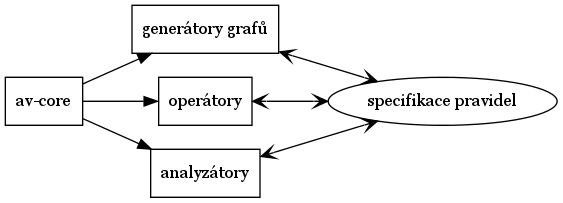
\includegraphics[width=0.8\textwidth]{./graphs/system_extensions.png}
  \caption{Body rozšíření systému.\label{design-system_extensions}}
\end{figure}

Vzhledem k~formalismu navrženému v~sekci \ref{design-graph_formalization} je nutné nejprve vhodným způsobem zpracovat vstup. K~tomu budou sloužit \emph{generátory grafů}. Jejich zodpovědností bude vygenerování určitého typu grafu z~AST analyzovaného programovacího jazyka.

Rozšíření typu \emph{operátor} představuje jeden konkrétní operátor (selektor nebo predikát), který je možné použít v~rámci \emph{souboru definic}. Každý operátor bude deklarovat své jméno, vstupy a výstupy.

Protože ne všechny kontroly zdrojového kódu lze zapsat jako pravidla s~výsledkem \verb+true+ nebo \verb+false+, bude možné do systému vložit vlastní \emph{analýzu}, jejímž vstupem bude graf konkrétního typu. Nad tímto grafem bude analýza vyhodnocena a výstup ve vhodném vnitřním formátu bude předán výstupnímu modulu.

Nyní můžeme již specifikovat rozhraní, která budou muset být implementována poskytovateli služeb (service providers):

\begin{itemize}
\item \emph{GraphGeneratorIface} -- rozhraní generátoru grafu,
\item \emph{OperatorIface} -- rozhraní operátorů (selektorů a predikátů),
\item \emph{AnalysisIface} -- rozhraní analytických modulů.
\end{itemize}

Celá dekompozice provedená v~tomto stupni je zachycena v~diagramu komponent na obrázku \ref{design-modules}. Modul jádra nazveme \verb+av-core+.
\begin{figure}[h!]
  \centering
  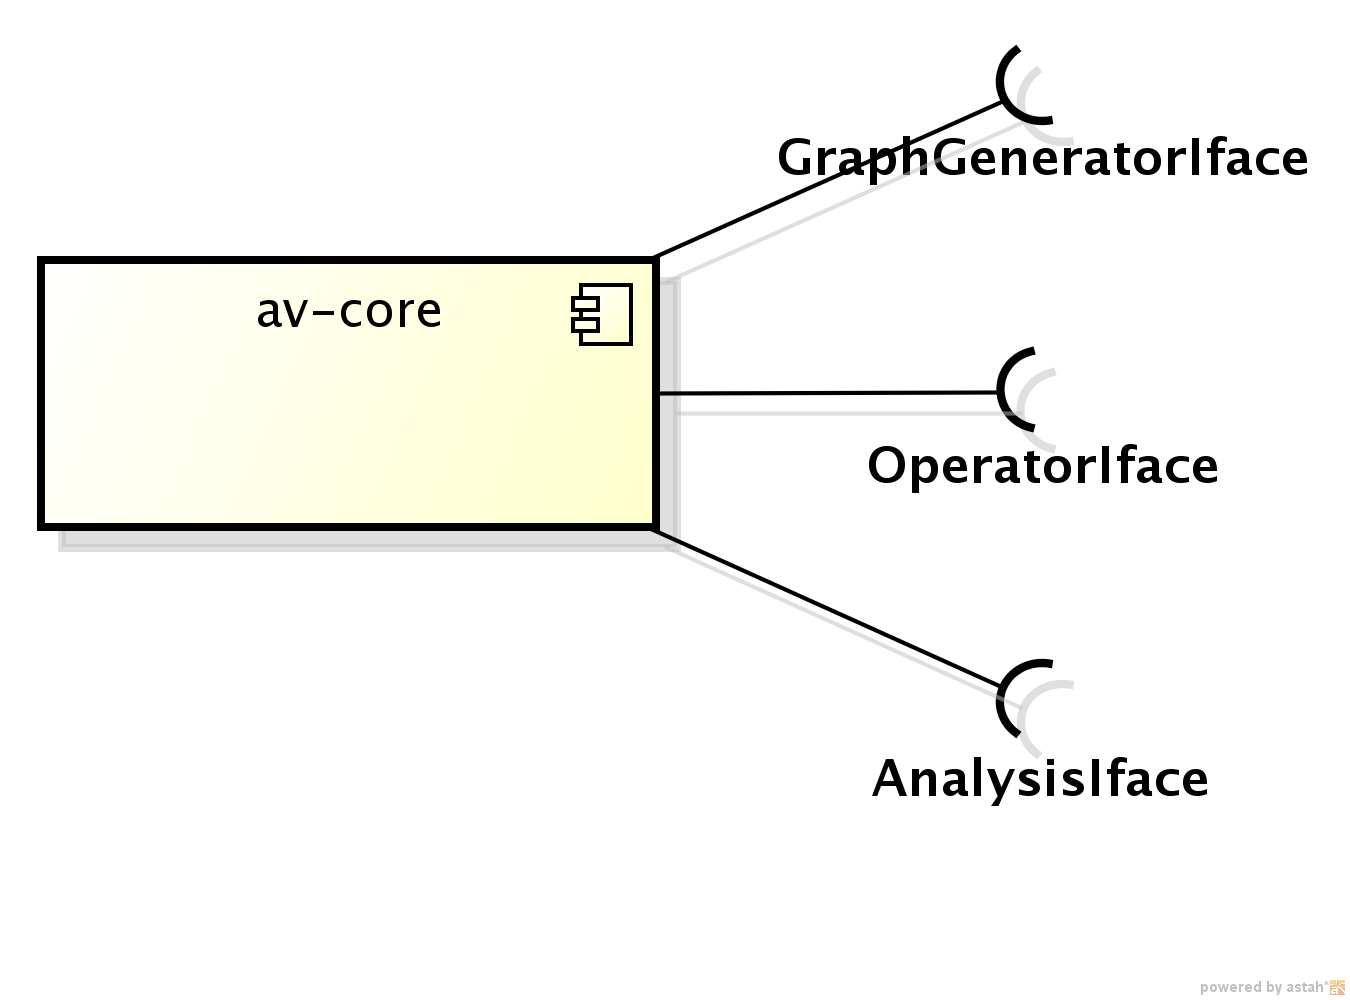
\includegraphics[width=0.5\textwidth]{./uml/archval_module_cmp.png}
  \caption{Dekompozice systému na jádro a rozšíření.\label{design-modules}}
\end{figure}
Jeho dekompozice bude provedena v~dalších sekcích. Ještě předtím se ale podíváme na důležité doménové objekty, které budou reprezentovat data předávaná mezi jednotlivými komponentami v~rámci systému.

\subsection{Doménové objekty}
\label{design-domain_objects}

Přehled doménových objektů podává tabulka \ref{design-domain_object_table}. Protože jsou tyto objekty součástí jádra a změna jejich rozhraní by nutně vedla k~úpravě ostatních komponent, navrhujeme tyto datové typy jako konkrétní třídy\footnote{U ostatních komponent předpokládáme, že budou implementovány třetími stranami. Je třeba pro ně třeba přesně definovat veřejná rozhraní SPI.}.

\begin{table}[h]
  \caption{Tabulka doménových objektů. \label{design-domain_object_table}}
  \begin{center}
    \begin{tabular}{| l | c | p{8cm} |}
      \hline
      \textbf{Název} & \textbf{Typ} & \textbf{Zodpovědnost} \\
      \hline
      \hline
      \emph{Graph} & class & graf reprezentující analyzované elementy \\ \hline
      \emph{Vertex} & class &  vrchol grafu \\ \hline
      \emph{Edge} & class & hrana grafu \\ \hline
      \emph{GraphModel} & class & množina grafů různých typů \\ \hline
      \hline
      \emph{ValidationModel} & class & model validace načtený ze vstupního \emph{souboru definic} \\ \hline
      \hline
      \emph{ValidationReport} & class &  objekt reprezentující výstup validace\\ \hline
      \emph{AnalysisReport} & class & objekt reprezentující výstup analýzy \\ \hline
    \end{tabular}
  \end{center}

\end{table}

Třídy \emph{ValidationModel} a \emph{GraphModel} je možné vygenerovat a používat opakovaně (cache). To se může hodit v~případech, kdy chceme tentýž projekt (pro nějž jsme již jednou generovali graf) validovat pomocí jiné/upravené množiny pravidel nebo naopak pokud chceme použít jednu množinu pravidel pro validaci více projektů. Bylo by zbytečné opakovaně provádět náročné operace generování grafu nebo parsování souboru pravidel a navazování operátorů (popisováno dále).

% TODO: zapracovat
ValidationModel v~sobě bude zapouzdřovat data z~AVD souborů. AVD soubory budou mít samostatné jmenné prostory pro následující typy jmen:

\begin{itemize}
\item názvy analýz
\item jména typů grafů
\item jména atomických a složených pravidel (jmenný prostor pro atomická i složená pravidla je sdílený)
\item jména operátorů
\end{itemize}

\subsubsection{Reprezentace grafů}
% TODO: rozepsat
\begin{itemize}
\item \emph{Graph} (class) -- graph type id
\item \emph{Vertex} (class)
\item \emph{Edge} (class)
\item \emph{GraphModel} (class) -- množina grafů různých typů, každý graf bude zahrnut právě jednou
\end{itemize}

\subsubsection{Model validace}
Model validace bude reprezentován třídou \emph{ValidationModel}. Tato třída bude reprezentovat existující množinu pravidel a současně bude umožňovat tato pravidla provést nad existující množinou grafů (\emph{GraphModel}).
% TODO: rozepsat
\begin{itemize}
\item \emph{ValidationModel} (class) -- AST strom souboru pravidel s~navázanými operátory; bude se přegenerovávat při úpravě souboru/textu v~GUI, atd\ldots
\end{itemize}

\subsubsection{Výstupní objekty}
% TODO: rozepsat, zpřesnit
\begin{itemize}
\item \emph{ValidationReport} (class) -- výstupem jsou \verb+true/false+ hodnoty pro jednotlivá pravidla, případně strom, který bude odpovídat stromu, který bude ve ValidationModel, aby bylo možné zpětně určit množiny a predikáty, které způsobily nesplnění pravidla
\item \emph{AnalysisReport} (class) -- výstupem budou tvrzení o~projektu, která budou doplněna množinami, pro která tato tvrzení platí (např. detekce anomálií -- projekt má příliš mnoho vazeb z~nějaké třídy do jiné)
\end{itemize}

\subsection{Jádro systému}
Jádro systému bude poskytovat třídy a rozhraní popsané v~tabulce \ref{design-archval_core_components}.

\begin{table}
  \caption{Tabulka komponent jádra systému. \label{design-archval_core_components}}
  \begin{center}
    \begin{tabular}{ | l | l | p{7.5cm} | }
      \hline
      \textbf{Název} & \textbf{Typ} & \textbf{Zodpovědnost} \\
      \hline
      \hline
      \emph{GraphModelGenerator} & class & zinicializuje jednotlivé moduly pro generování grafů a použije je pro vygenerování grafů (pokud jsou tyto grafy požadovány) \\ \hline
      \emph{GraphModelGeneratorIface} & interface & rozhraní předchozí komponenty \\ \hline
      \emph{ValidationModelGenerator} & class & generátor, který na základě validační specifikace vygeneruje instanci třídy \mbox{\emph{ValidationModel}} \\ \hline
      \emph{ValidationModelGeneratorIface} & interface & rozhraní předchozí komponenty \\ \hline
      \emph{ValidationTask} & class & hlavní proces validace \\ \hline
      \emph{ValidationTaskIface} & interface & rozhraní předchozí komponenty \\ \hline
      \emph{Validator} & class & bude provádět validaci pravidel v~grafu na základě vstupních pravidel \\ \hline
      \emph{Analyzer} & class & bude provádět statistické analýzy (pro návrhové principy, které nelze popsat přesnými pravidly) \\ \hline
      \emph{ArchVal} & class & fasáda ArchVal systému -- bude poskytovat instance výše specifikovaných komponent \\ \hline
      \hline
      \emph{GraphGeneratorsRegisterIface} & interface & rozhraní registru existujících poskytovatelů generátorů grafu \\ \hline
      \emph{OperatorsRegisterIface} & interface & rozhraní registru existujících poskytovatelů operátorů \\ \hline
      \emph{AnalysesRegisterIface} & interface & rozhraní registru poskytovatelů komponent analýzy \\ \hline
    \end{tabular}
  \end{center}

\end{table}

\begin{itemize}
\item \emph{GraphModelGenerator} -- updateGraphModel() -- přegeneruje graph model -- pouze doplní požadované chybějící grafy, regenerate() -- kompletně zruší všechny grafy a vygeneruje nové (všechny požadované)
\end{itemize}

Na obrázku \ref{design-archval_core} jsou zobrazeny komponenty modulu \emph{archval-core}.

% TODO: připsat k rozhraní graph generator:
Reprezentuje komponentu, která provede převod zdrojových kódů na graf (zobrazení, které vybraným elementům AST přiřadí množinu vrcholů $V$ grafu $G$).

\begin{figure}[h!]
  \centering
  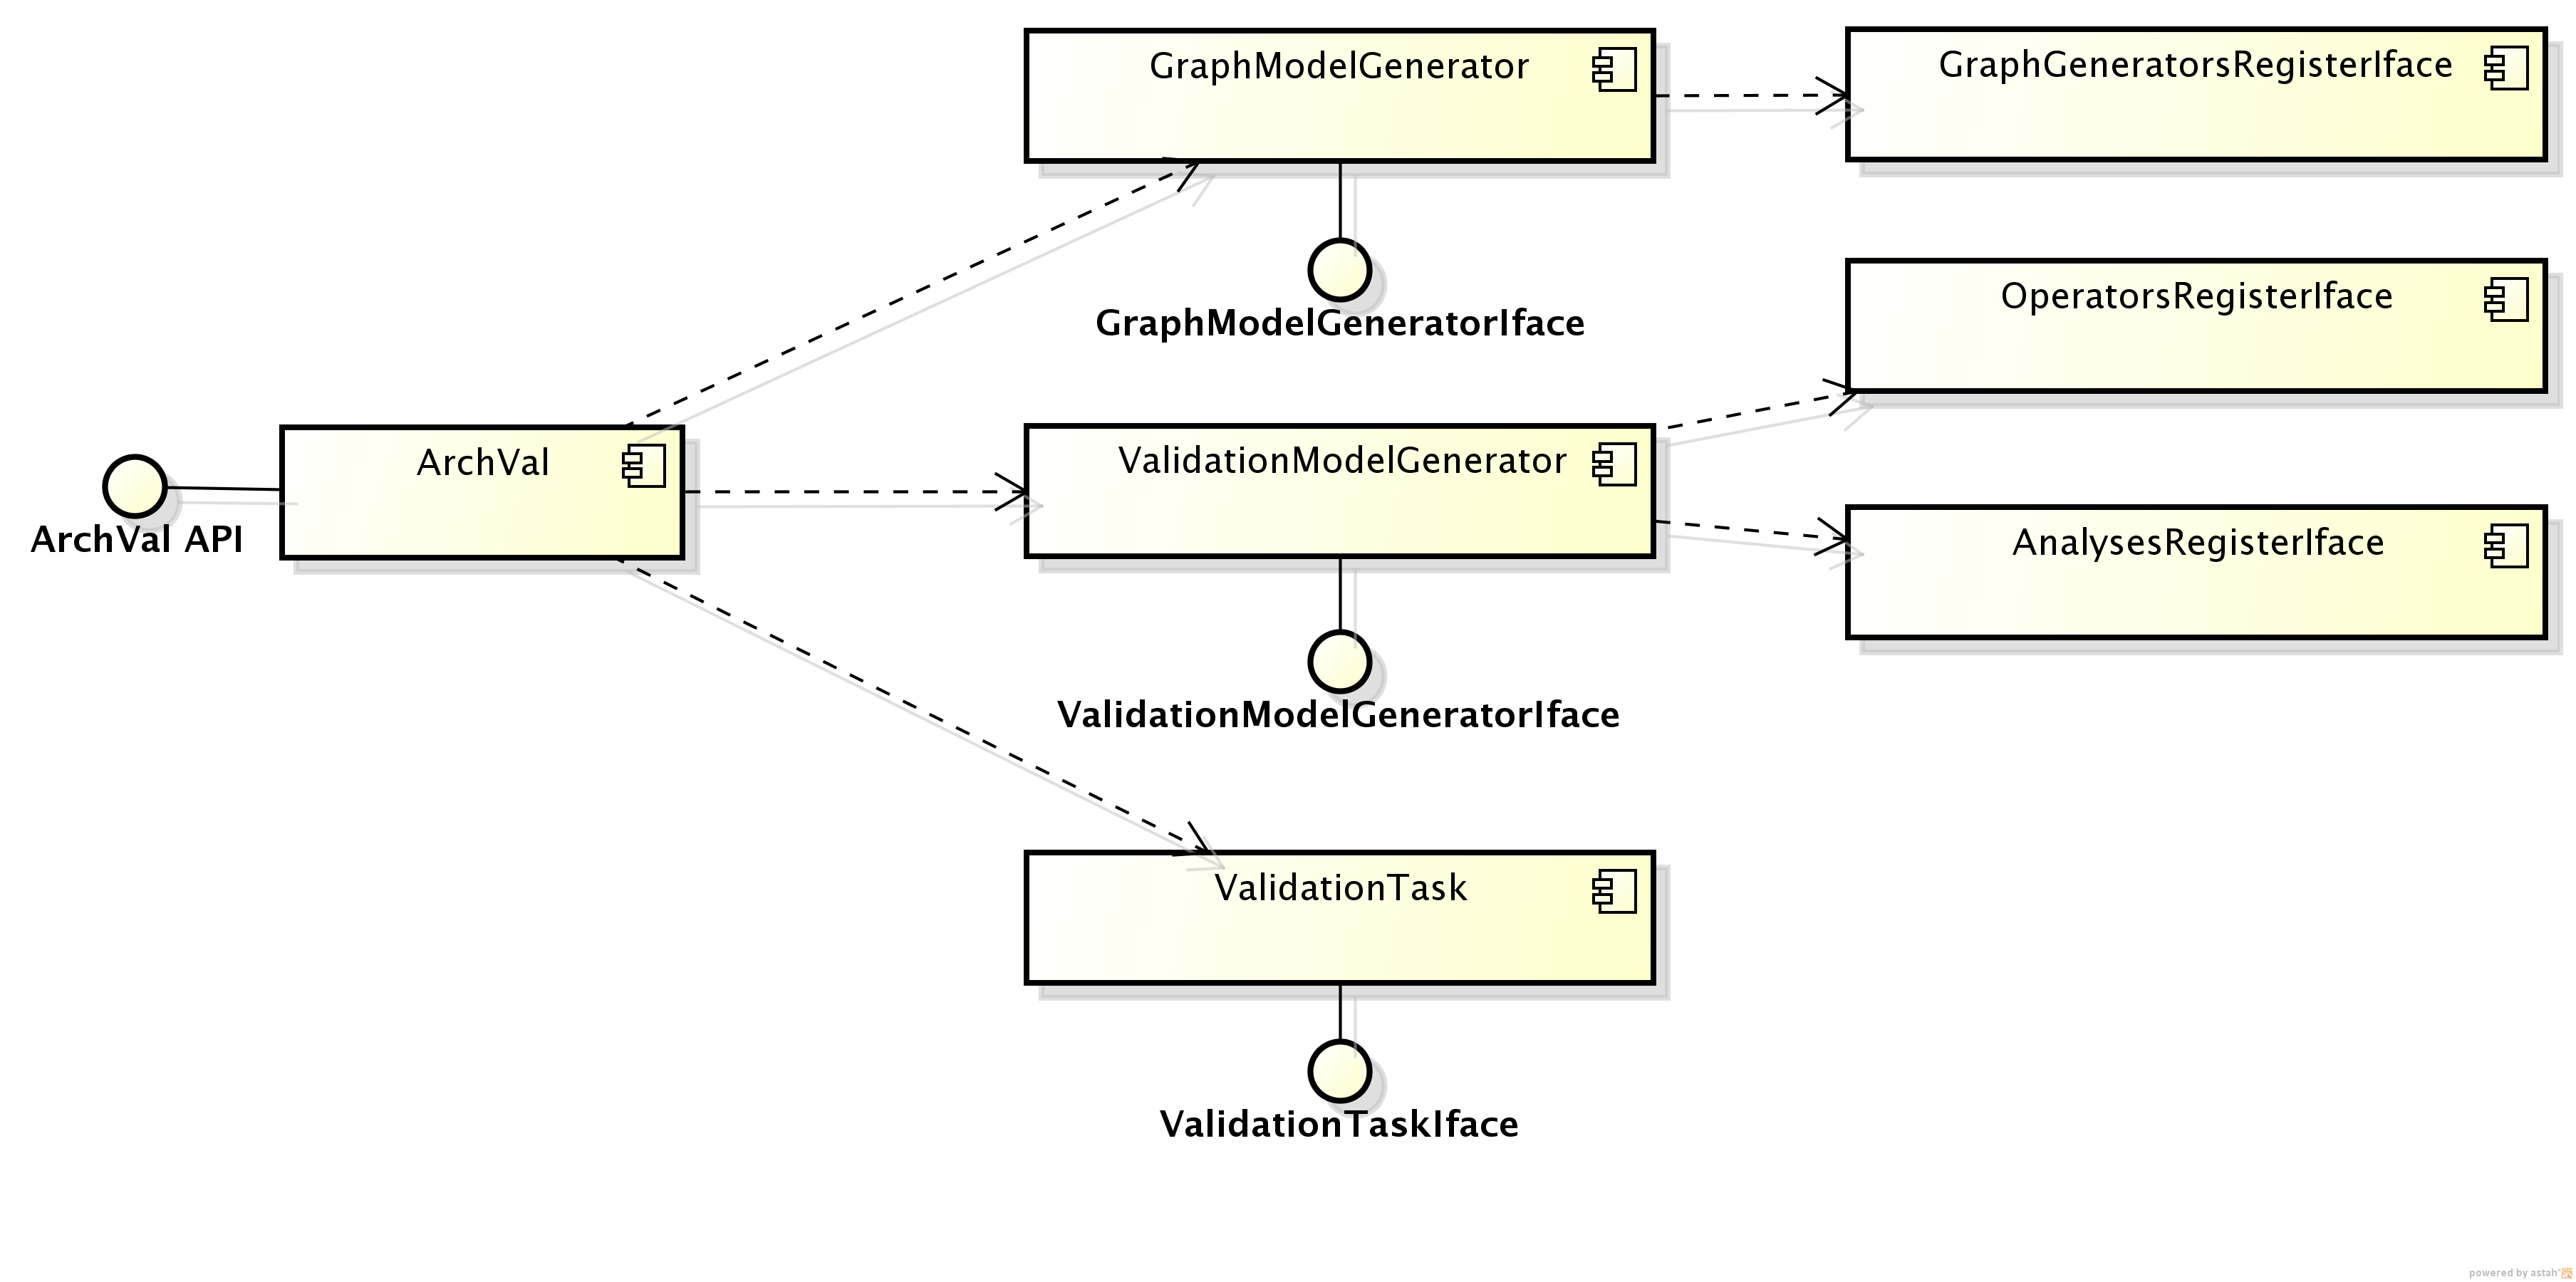
\includegraphics[width=1.0\textwidth]{./uml/archval_core_cmp.png}
  \caption{Komponenty jádra systému ArchVal.\label{design-archval_core}}
\end{figure}

\subsubsection{Komponenta GraphModelGenerator}
% TODO: rozepsat
GraphModelGeneratorIface

Komponenta typu \emph{GraphModelGeneratorIface} je znázorněna na obrázku \ref{design-graph_generator_io}.

\begin{itemize}
\item \emph{Vstup:} seznam Java souborů, z~nichž sestává projekt, identifikátory požadovaných typů grafů
\item \emph{Výstup:} GraphModel objekt
\end{itemize}

\begin{figure}[h!]
  \centering
  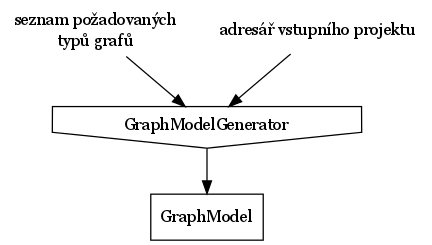
\includegraphics[width=0.55\textwidth]{./graphs/graph_generator_io_graph.png}
  \caption{Znázornění vstupů a výstupů komponenty typu \emph{GraphModelGenerator}.\label{design-graph_generator_io}}
\end{figure}

\subsubsection{Komponenta ValidationModelGenerator}
% TODO: formulate
ValidationModelGeneratorIface

Znázornění vstupů a výstupů komponenty \emph{ValidationModelGenerator} je na obrázku \ref{design-validation_model_generator_io}.

% TODO: zkontrolovat, že 'výše popsaných pravidel' odkazuje na nějaká předchozí pravidla dříve v práci
Vstupem je množina pravidel zapsaná ve vhodné serializaci výše popsaných matematických pravidel.

\begin{figure}[h!]
  \centering
  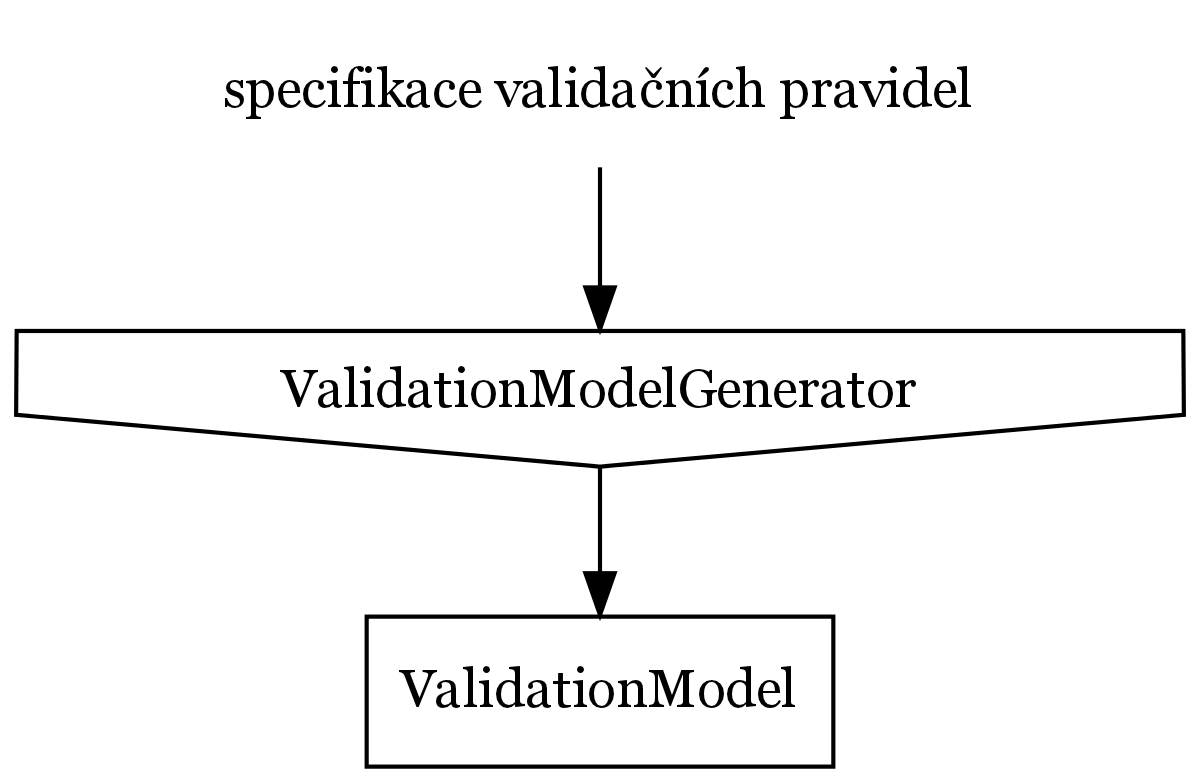
\includegraphics[width=0.55\textwidth]{./graphs/validation_model_generator_io_graph.png}
  \caption{Znázornění vstupů a výstupů komponenty \emph{ValidationModelGenerator}.\label{design-validation_model_generator_io}}
\end{figure}

Různé vstupy: File, Stream, String, \ldots

\subsubsection{Komponenta ValidationTask}
ValidationTaskIface

Samostatné vlákno s~řízením celého validačního procesu. Synchronized sekce. Vstupem bude vhodná specifikace umístění analyzovaného projektu.

% TODO: vyladit a doplnit následující interface
\begin{itemize}
\item \verb+setProject()+
\item \verb+startValidationThread()+
\item \verb+cancelValidationThread()+
\item \verb+getReport()+
\item \verb+runSynchronous()+
\item \verb+runAsynchronous()+
\item \verb+addProgressListener(ValidationTaskProgressListener)+ -- umožní zaregistrovat listener, který bude notifikován o~průběhu validace
\end{itemize}

\subsubsection{Komponenta Validator}
Vstupem bude ValidationModel a GraphModel

Komponenta \emph{Validator} je znázorněna na obrázku \ref{design-validator_io}.

\begin{figure}[h!]
  \centering
  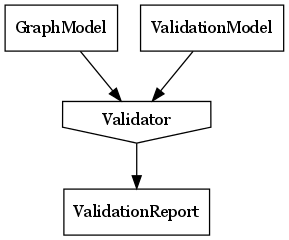
\includegraphics[width=0.45\textwidth]{./graphs/validator_io_graph.png}
  \caption{Znázornění vstupů a výstupů komponenty \emph{Validator}.\label{design-validator_io}}
\end{figure}

\paragraph{Rozhraní}
\begin{itemize}
\item \verb-+performValidation(ValidationModel, GraphModel) : ValidationReport-
\end{itemize}

Výstupem bude \emph{ValidationReport} (vnitřní struktura, která se bude posléze převádět na vhodnou vnější reprezentaci).

\subsubsection{Komponenta Analyzer}
\begin{itemize}
\item analysis providers
\item vstupem bude \emph{GraphModel} -- musí specifikovat nad jakým grafem pracuje
\item výstupem bude \emph{AnalysisReport}
\end{itemize}

\subsubsection{Rozhraní registrů poskytovatelů implementací}

Aby bylo možné systém rozšiřovat přidáváním dalších operátorů, generátorů grafů nových typů a analýz, musíme poskytnout vhodný mechanismus, který umožní zapojení nových modulů do programu.
% TODO: sort
\begin{itemize}
\item SPI, poskytovatel služby, lookup, META-INF/services,
\end{itemize}

\begin{itemize}
\item GraphGeneratorsRegisterIface
\item OperatorsRegisterIface
\item AnalysesRegisterIface
\end{itemize}

\subsubsection{Komponenta ArchVal (fasáda)}
% TODO: napsat, jakým způsobem bude fungovat (v podstatě singleton)
\paragraph{Rozhraní}
\begin{itemize}
\item \verb-+createValidationTask(ValidationModel, GraphModel) : ValidationTask-
\item \verb-+getGraphModelGenerator() : GraphModelGenerator-
\item \verb-+getValidationModelGenerator() : ValidationModelGenerator-
\end{itemize}

\subsection{Rozhraní GraphGeneratorIface}
% TODO: roztřídit
%% \item compiler
%% \item generátor vnitřní struktury (modelu) -- modelem je v našem případě graf
%%   \begin{itemize}
%%   \item \emph{vstup:} množina cest k \verb+*.java+ souborům (kompilačním jednotkám), z nichž se skládá softwarový projekt
%%   \item \emph{výstup:} graf, reprezentující konkrétní analyzovanou doménu vhodný pro další zpracování (graf podle \ref{design-graph_formalization} \nameref{design-graph_formalization})
%%   \end{itemize}
\begin{itemize}
\item \emph{vstup:} vhodná reprezentace zdrojových kódů projektu (např. seznam všech souborů)
\item \emph{výstup:} graf konkrétního typu (např. demeter graph)
\end{itemize}

Každý graph generátor (resp. graf) musí mít specifikované jedinečné id grafu. (To bude dále použito např. při specifikaci pravidel, kde je potřeba sdělit validátoru, nad kterým grafem má pravidlo platit).

\begin{itemize}
\item \verb+getGraphTypeId() : String+
\item \verb+generateGraph(projectFilesSpecification) : Graph+
\end{itemize}

\subsection{Rozhraní OperatorIface}
Hierarchie rozhraní operátorů je znázorněna na obrázku \ref{design-operator_interfaces_hierarchy}.

\begin{itemize}
\item \emph{PredicateIface}
\item \emph{VertexSelectorIface}
\item \emph{EdgeSelectorIface}
\end{itemize}

\begin{figure}[h!]
  \centering
  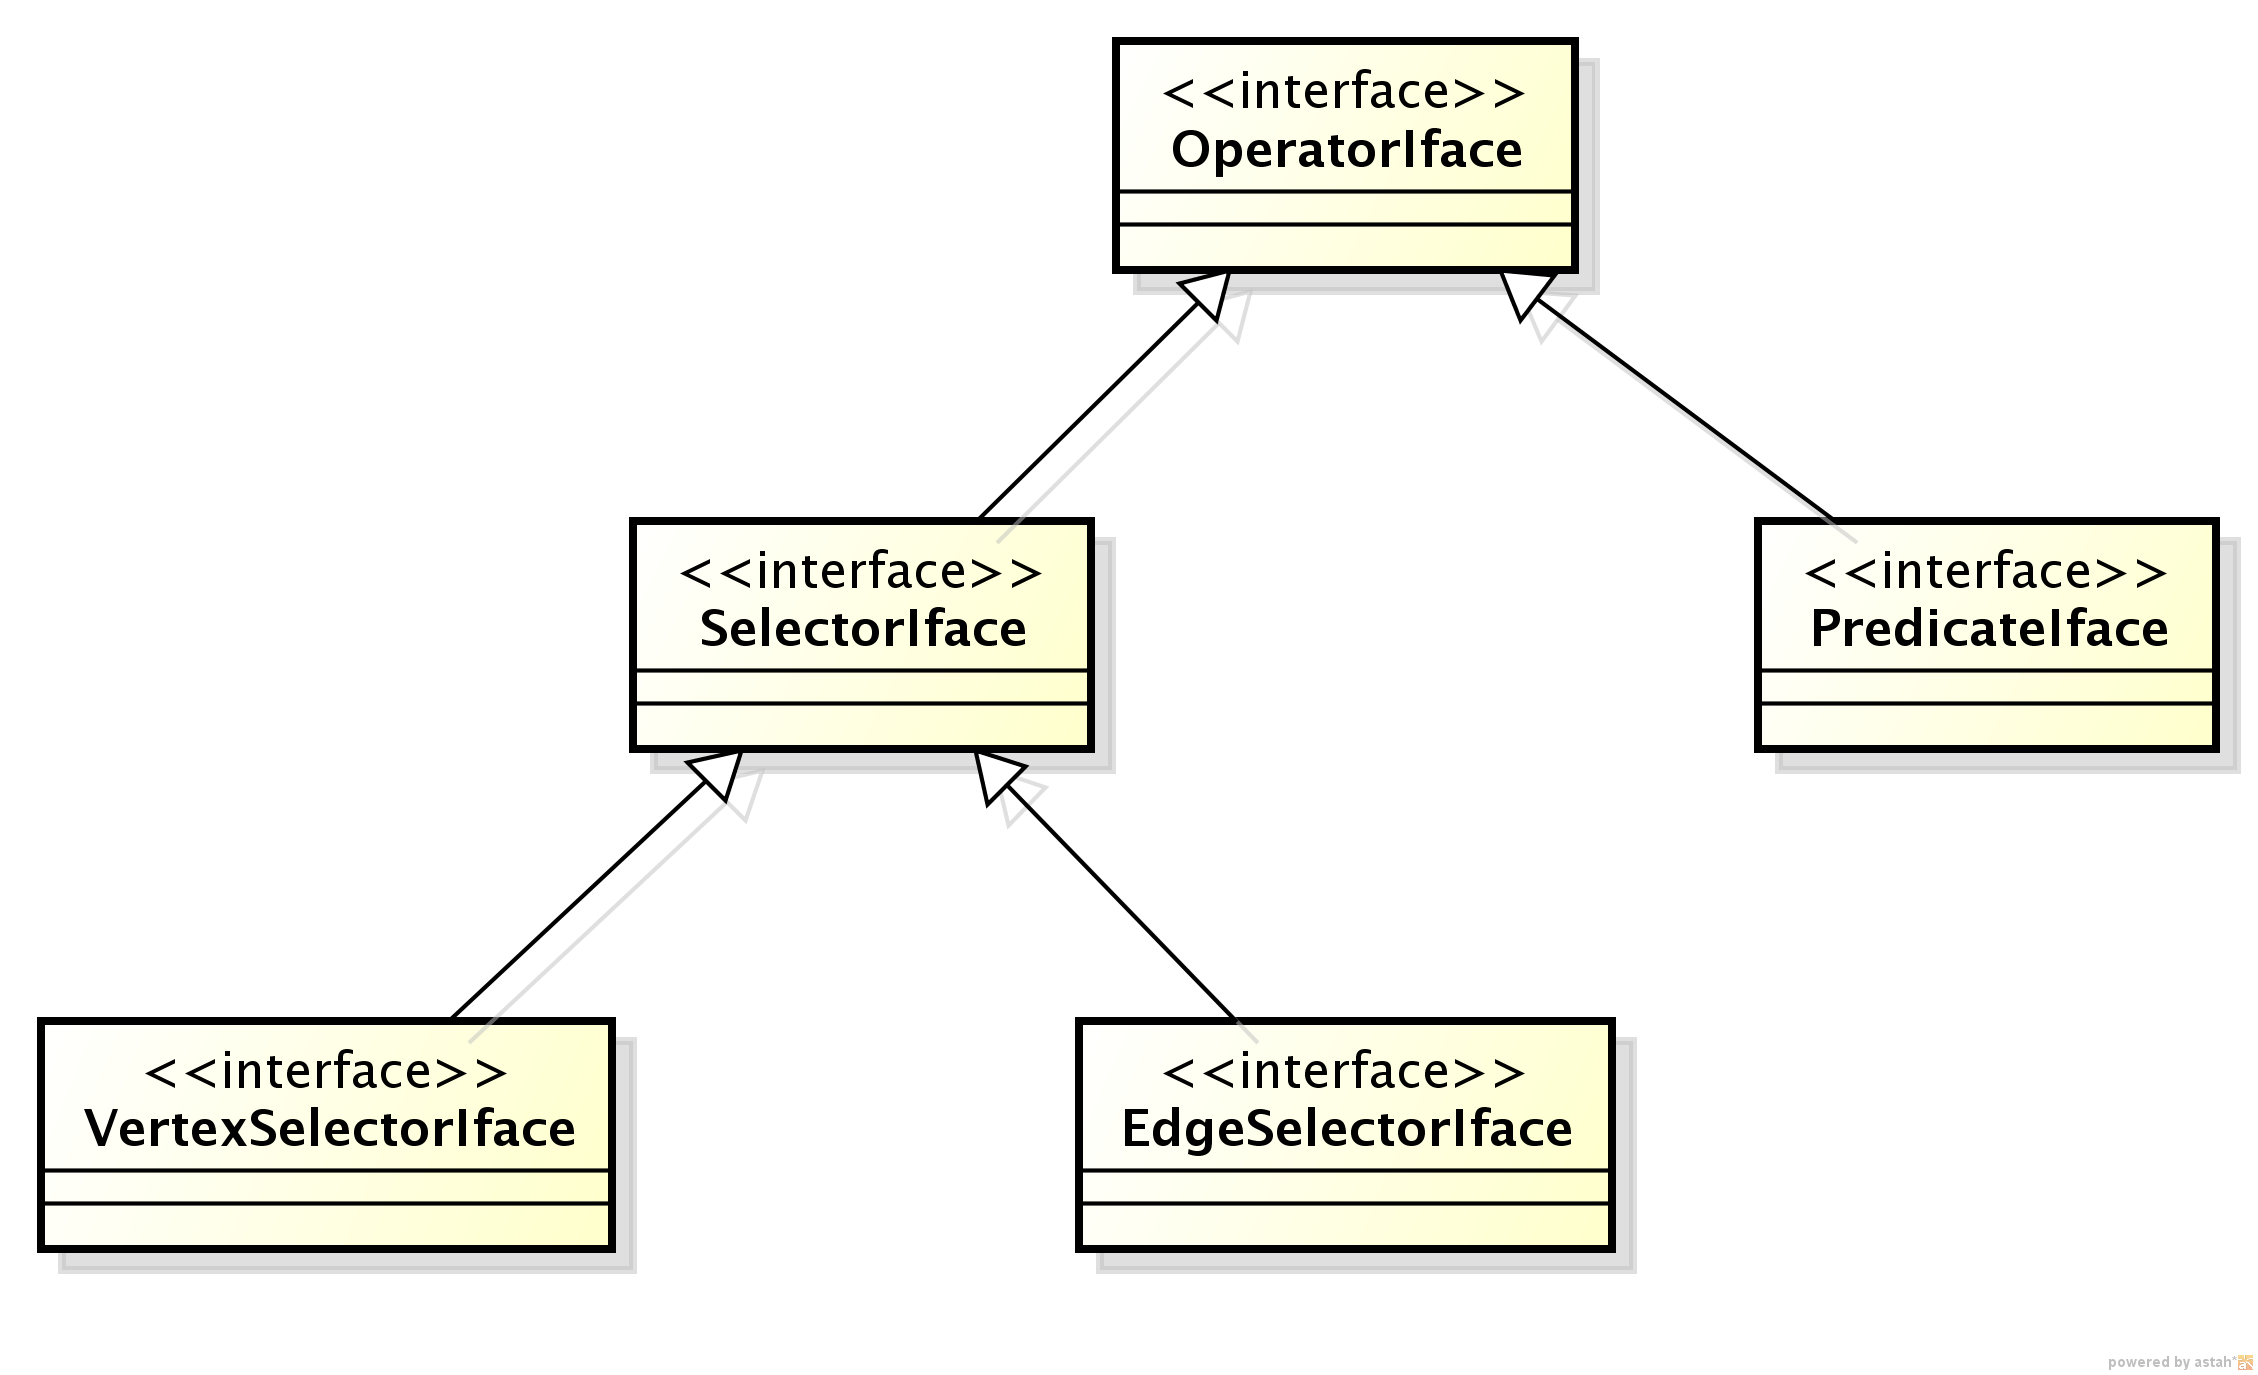
\includegraphics[width=0.8\textwidth]{./uml/operator_interfaces.png}
  \caption{Hierarchie rozhraní operátorů.\label{design-operator_interfaces_hierarchy}}
\end{figure}

\subsection{Rozhraní AnalysisIface}

\subsection{Základní průběh validačního procesu}

%% TODO: zapracovat || přesunout || smazat
%% * source code references resolution/resolving
%% * dependency graph construction
%% * dependency graph visualization
%% * GUI design and implementation
%% * graph analysis
%% * graph data mining

%TODO: add activity and/or sequence diagram
%TODO: popis validačního procesu: rozepsat následující itemize
\begin{itemize}
\item systém načte moduly
\item systém zkontroluje základní předpoklady - existuje alespoň jeden modul pro generování grafu, alespoň jeden modul operátorů (nebo poskytovatel analyzerů ???) a alespoň jeden modul s~poskytovatelem generátoru výstupu
\item systém zparsuje soubor pravidel a vygeneruje AST
\item systém zkontroluje, zda pro AST pravidel existují potřebné providery grafů
\item systém zkontroluje, zda pro AST pravidel existují všechny operátory
\item systém provede nabindování operátoru na uzly AST pravidel
\item systém vygeneruje pro projekt všechny požadované grafy
\item systém vyhodnotí AST nad grafy pomocí operátorů, zjištěná porušení pravidel bude zapisovat do validačního reportu
\item systém projde všechny analyzátory a nechá je vygenerovat analyzační report
\item systém pomocí výstupních modulů vygeneruje reporty (na základě konfigurace ???)
\end{itemize}

\section{Návrh rozhraní pro zadávání pravidel}
%% TODO: zapracovat:
U~každého pravidla musí být deklarace typu grafu, nad nímž má platit.
%% rozhraní pro zadávání pravidel bude dáno jazykem, který se pro definici pravidel bude používat - možná kompilátor DSL jazyka, výrazy, atd.
\begin{itemize}
\item rozhraní pro zadávání pravidel
\item formát zadávání pravidel (serializace formalismu tak, aby jej bylo možné textově nebo jinak zadávat)
\item zvýrazňování syntaxe
\end{itemize}

\section{Návrh rozhraní pro ověřování platnosti pravidel (validaci)}
%% TODO: navrhnout způsob a formát výstupu
%% - diskutovat různé možnosti
%%     - textový výstup v okně
%%     - reprezentace swing komponentou
%%     - html výstup
%%     - výstup do souboru
\begin{itemize}
\item výstupní rozhraní
\item validační události
\end{itemize}

\section{Návrh způsobu integrace do různých typů prostředí}
%% TODO: zapracovat
%% návrh je řešen tak, aby bylo možné poskytnout další rozhraní k systému (např. CLI, TUI, atd.) - ValidationTask lze zabudovat do jiných programů a lze jej řídit, při poskytnutí rozhraní *Register je možné dodávat poskytovatele služeb i z jiných zdrojů (na platformě NetBeans je řešeno pomocí lookupů <- tohle patří ale spíš do implementace)

Rozhraní ArchVal API je záměrně navrženo tak, aby jej bylo možné integrovat do různých typů prostředí, např:

\begin{itemize}
\item CLI -- skripty, readline, atd.
\item TUI -- jednoduché textové rozhraní pro validaci
\item GUI -- zde NetBeans platforma
\end{itemize}

Možnosti různého způsobu vstupu pravidel -- editor se zvýrazňováním syntaxe.

\section{Návrh technologií pro implementaci}
\begin{itemize}
\item NetBeans platform
\item Maven project
\item Java 1.6
\item vstupem bude Java Maven projekt
\item \ldots
  % TODO: vytvorit prehled technologii i s jejich popisy
\end{itemize}
